%マルチサイクルテスト
本章では,マルチサイクルテストの概要と,
マルチサイクルテストにおける縮退故障の検出および遅延故障の検出に関してそれぞれ述べる.

%1節
\section{マルチサイクルテスト}
マルチサイクルテスト\cite{multicycle}とは,スキャンテストにおいて
複数回のキャプチャサイクルを繰り返す手法である.
LoC方式に対してマルチサイクル化を施した場合のタイミングチャートを図3.1に示す.

\begin{figure}[h]
	\begin{center}
		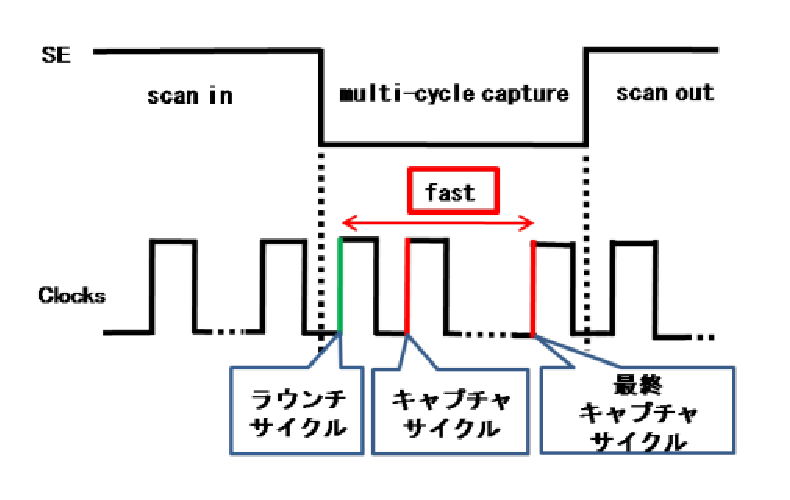
\includegraphics[height=50mm]{LoCmulti.eps}
		\caption{マルチサイクルによるLoCのタイミングチャート}
	\end{center}
\end{figure}

マルチサイクルテストでは,スキャンシフト動作でテストパターンをスキャンチェーンに設定した後,
通常動作で,システムクロックによりキャプチャを行い,テスト応答としてスキャンチェーンに値が設定される.
その後,2サイクル目のテストモードにおいて,再度キャプチャを行い,
テスト応答がスキャンチェーンに設定される.
このように,キャプチャを繰り返し最終キャプチャで得られた値をスキャンアウトすることで,
テストパターンに対するテスト応答を確認する手法である.

マルチサイクルテストの時間実行例としてサイクル数を3とした場合の例を図3.2に示す.
まず,スキャンイン動作で(110)が入力される.
1サイクル目でキャプチャされたパターン(001)を入力として2サイクル目が実行される.
2サイクル目でキャプチャされたパターン(101)を入力として3サイクル目が実行される.
3サイクル目でキャプチャされたパターン(101)をスキャンアウトすることでテスト結果を得る.

\begin{figure}[h]
	\begin{center}
		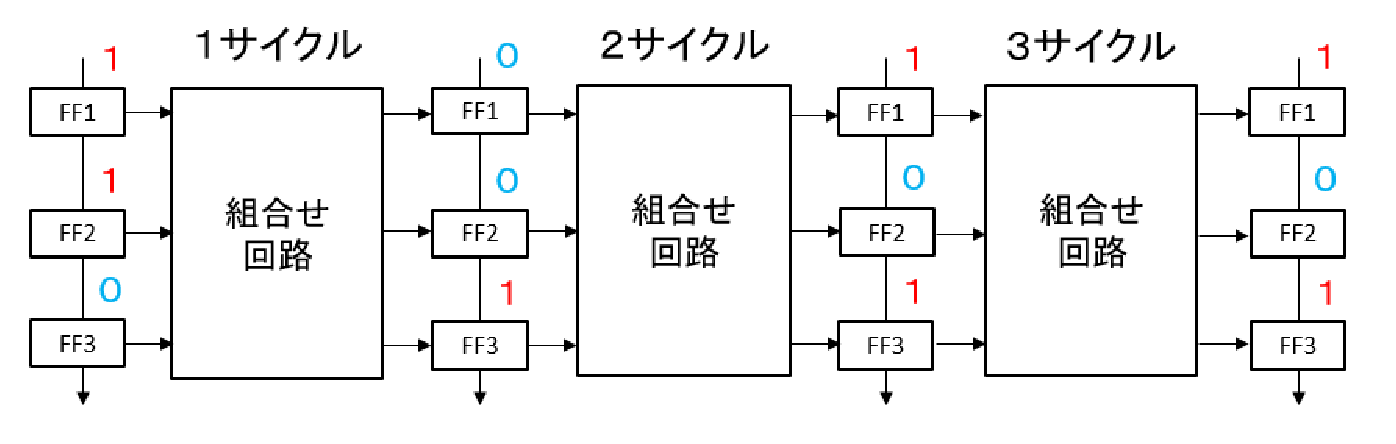
\includegraphics[height=40mm]{multicycle.eps}
		\caption{マルチサイクルテスト}
	\end{center}
\end{figure}	

マルチサイクルテストでは,各サイクルでキャプチャされたパターンを
次のキャプチャサイクルのテストパターンとして再利用することで,
従来のスキャンテストと比較したときに,テストパターンの生成数を抑えつつ
より多くの故障検出を行う機会を獲得できる.

%2節
\section{マルチサイクルテストにおける故障検出}

%2節1項
\subsection{マルチサイクルテストにおける縮退故障の検出}
ここでは,マルチサイクルテストにおける縮退故障の検出に関して述べる.
ある信号線Lの0(1)縮退故障を検出するためには,
テストパターンによってその信号線Lに1(0)を設定することで故障が励起される.
次に,この縮退故障の影響が被検査回路の出力側のフリップフロップにおいて
誤り論理値として取り込まれることによって,
テストパターンによって縮退故障が検出できたと判定する.

図3.3にマルチサイクルテストにおける縮退故障の検出例を示す.

\begin{figure}[h]
	\begin{center}
		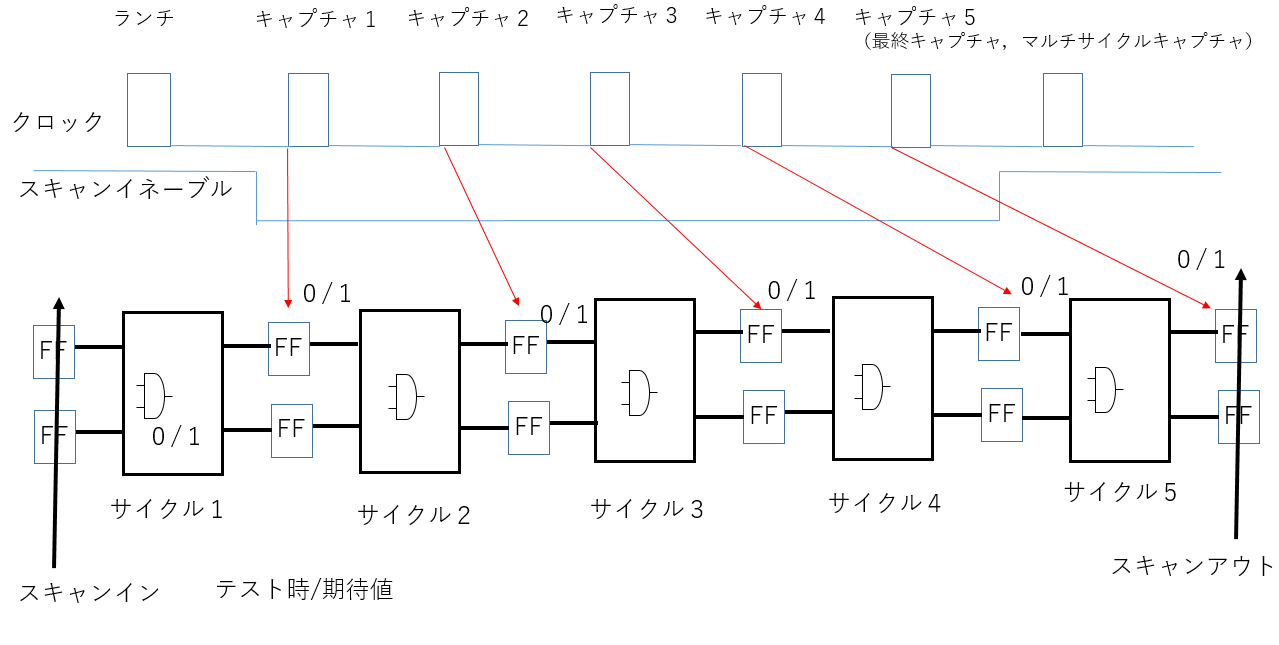
\includegraphics[height=70mm]{degenetest.eps}
		\caption{マルチサイクルテストにおける縮退故障の検出例}
	\end{center}
\end{figure}

マルチサイクルテストにおいては,まず,
スキャンフリップフロップにテストパターンがスキャンインされた後に,
被検査回路をシステムクロックのテストモードで動作させる.
次に,キャプチャクロックで1サイクル目のテストモードで回路が動作した結果として,
得られた応答がフリップフロップに取り込まれる.
図3.2の例では,2サイクル目以降のフリップフロップにおいて,
テスト時に取り込まれた論理値と期待値が異なるため,
最終サイクルのテストモードにおいて回路が動作した結果として
得られた応答がフリップフロップに取り込まれ,
テスト時に取り込まれた論理値と期待値が異なるため縮退故障が検出できたと判定する.

%2節2項
\subsection{マルチサイクルテストにおける遅延故障の検出}
ここでは,マルチサイクルテストにおける遅延故障の検出に関して述べる.
ある信号線Lの立ち下がり(立ち上がり)遅延故障を検出するためには,
まず,テストパターンによってその信号線Lに1(0)を初期値として設定し,
次のテストパターンによってその信号線Lに0(1)を設定することで,
立ち下がり(立ち上がり)遅延故障が励起される.
次に,この遅延故障の影響が被検査回路の出力側のフリップフロップにおいて
誤り論理値が取り込まれることによって,テストパターンによって遅延故障が検出できたと判定する.

図3.4にマルチサイクルテストにおける遅延故障の検出例を示す.

\begin{figure}[h]
	\begin{center}
		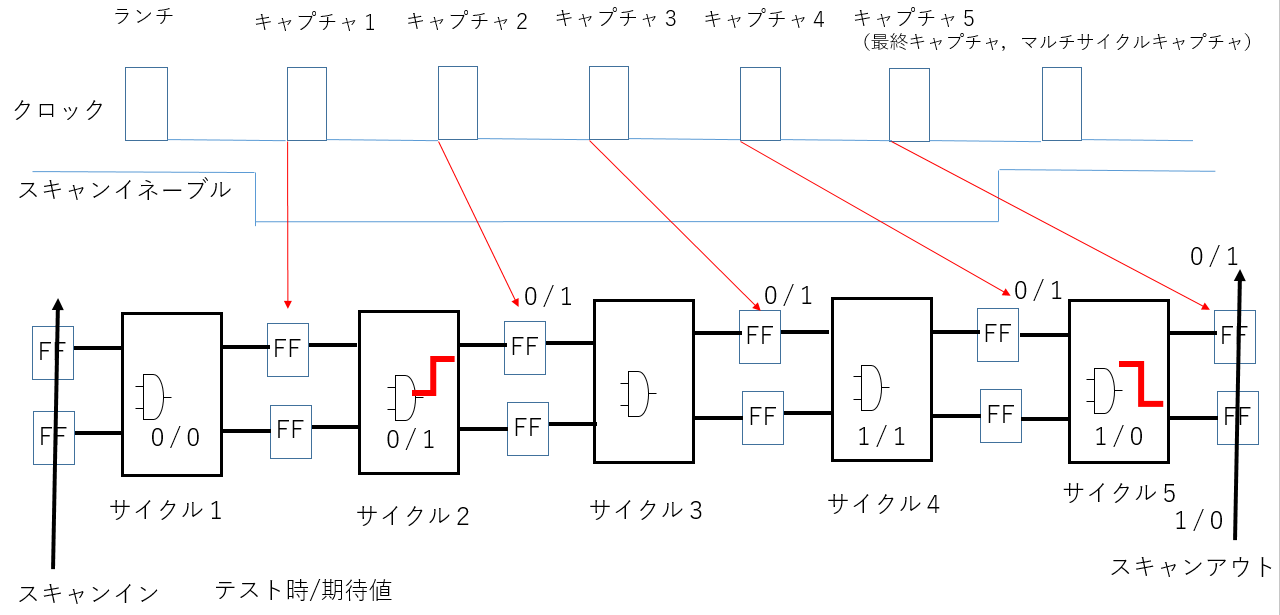
\includegraphics[height=70mm]{trantest.eps}
		\caption{マルチサイクルテストにおける遅延故障の検出例}
	\end{center}
\end{figure}

マルチサイクルテストにおいては,まず,
スキャンフリップフロップにテストパターンがスキャンインされた後に,
被検査回路をシステムクロックのテストモードで動作させる.
次に,キャプチャクロックで1サイクル目のテストモードで回路が動作した結果として,
対象とする信号線に初期値を設定している.
次に,2サイクル目のテストモードにおいて,
対象とする信号線に信号遷移(立ち上がり信号変化)を励起している.
対象とする信号線の信号遷移(立ち上がり信号変化)が遅延故障の影響を受けるので,
その遅延故障の影響が伝搬する出力側のフリップフロップにおいて誤り論理値が取り込まれる.
その誤り論理値の影響が最終サイクルまで伝搬することによって,遅延故障が検出できたと判定する.

さらに,図3.4では,4サイクル目に初期値1を設定し,
5サイクル目で対象とする信号線に信号遷移(立ち下がり信号変化)を励起し,
出力側のフリップフロップにおいて誤り論理値が取り込まれることで,遅延故障が検出できたと判定する.

%3節
\section{マルチサイクルテストにおける故障検出能力低下問題}
マルチサイクルテストには ``故障検出能力低下問題'' がある.
故障検出能力低下問題\cite{multidemerit}とは,キャプチャサイクルを重ねるにつれ
次第に新たな故障を検出しにくくなっていく問題である.
マルチサイクルテストでは,被検査回路の内部状態を機能動作に近づけることができ,
多数のキャプチャサイクル(20サイクル)を適用した場合,
被検査回路の内部状態遷移はサイクル数を増やすことによって低減することが報告されている\cite{FFtgl}.
多数のキャプチャサイクルを適用した場合における,
FFの内部状態遷移を示したグラフを図3.5に示す.
図の縦軸は,各FFの値がサイクル毎に遷移の発生した回数,横軸はサイクル数を示している.

\begin{figure}[h]
	\begin{center}
		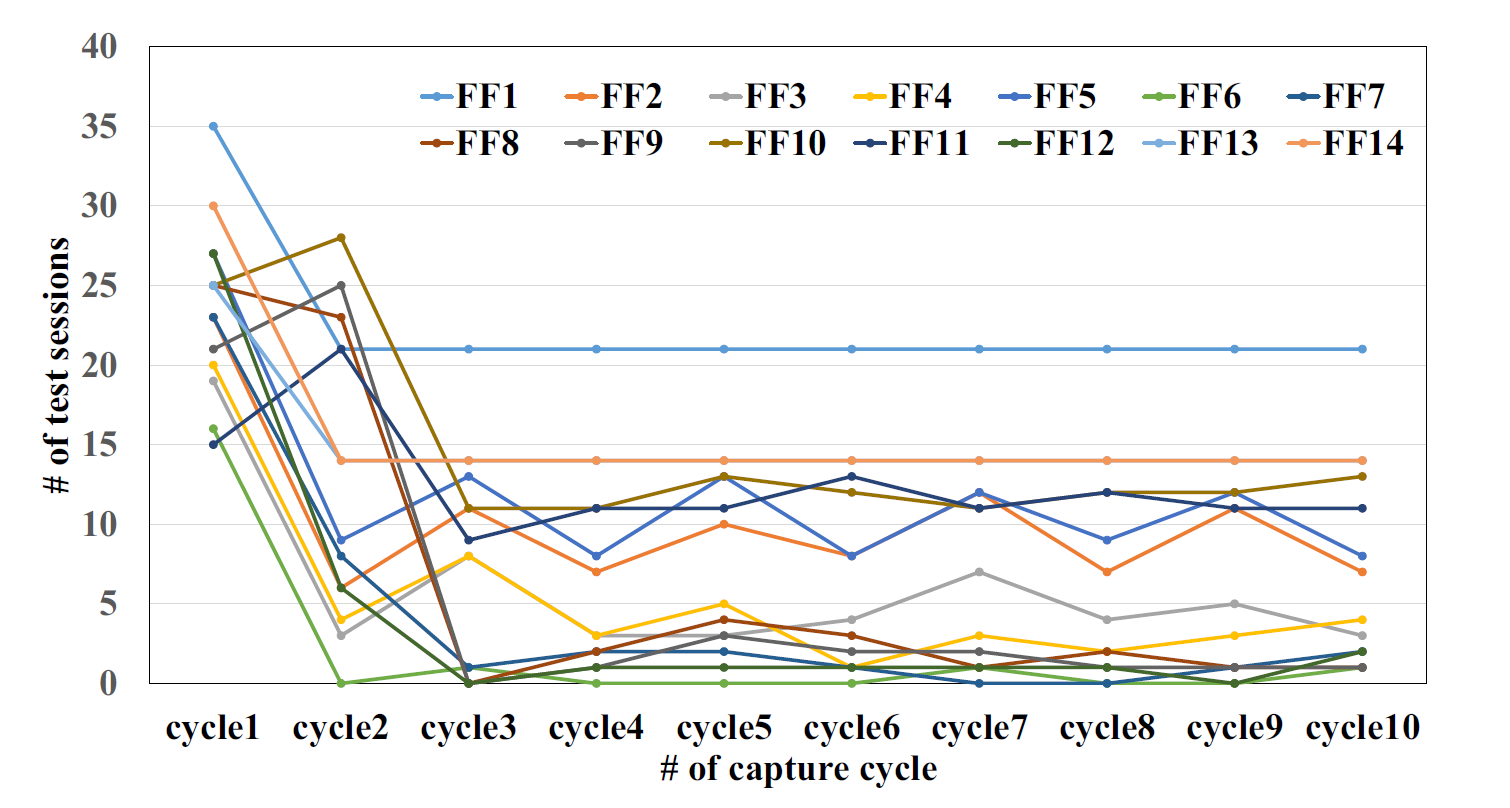
\includegraphics[height=70mm]{FFtgl.eps}
		\caption{マルチサイクルキャプチャによるFFの状態遷移回数変化(s298ベンチマーク回路)}
	\end{center}
\end{figure}

図から読み取れるように,サイクル数の増加に伴い各FFの内部状態の遷移回数は減少することから,
多数のキャプチャサイクルを適用した場合,FFの値は固定値となり,故障検出能力は低下する.

故障検出能力低下問題におけるFF固定値の例として,
サイクル数を3とした場合のマルチサイクルテストを図3.6に示す.

\begin{figure}[h]
	\begin{center}
		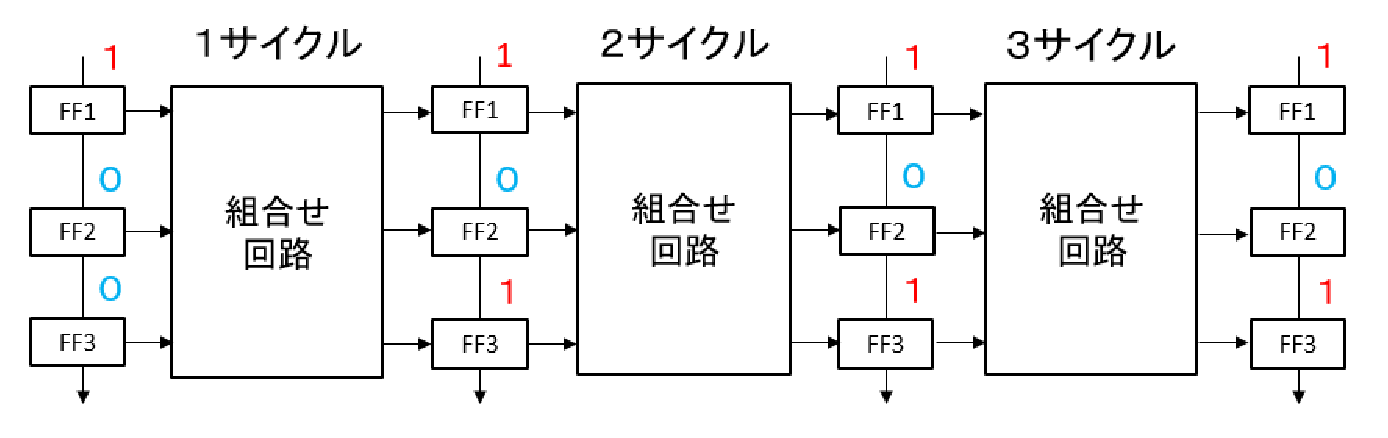
\includegraphics[height=40mm]{trandem.eps}
		\caption{マルチサイクルテストにおける故障検出能力低下問題}
	\end{center}
\end{figure}

まず,スキャンイン動作で(100)が入力される.
1サイクル目でキャプチャされたパターン(101)を入力として2サイクル目が実行される.
2サイクル目でキャプチャされたパターン(101)を入力として3サイクル目が実行される.
3サイクル目でキャプチャされたパターン(101)をスキャンアウトすることでテスト結果を得る.

このように,被検査回路の内部状態遷移の減少によって,
キャプチャパターンが最初のサイクルで適用されたテストパターンと比較して,
ランダム性の少ない入力パターンになってしまい,
新たな故障を検出する能力が低下する.
この問題を改善し,故障を検出する能力を向上させるため,
4章で説明するFF制御点挿入を用いて実験を行う.